\chapter{PMT Upgrade}

\begin{figure}
	\centerline{
		\mbox{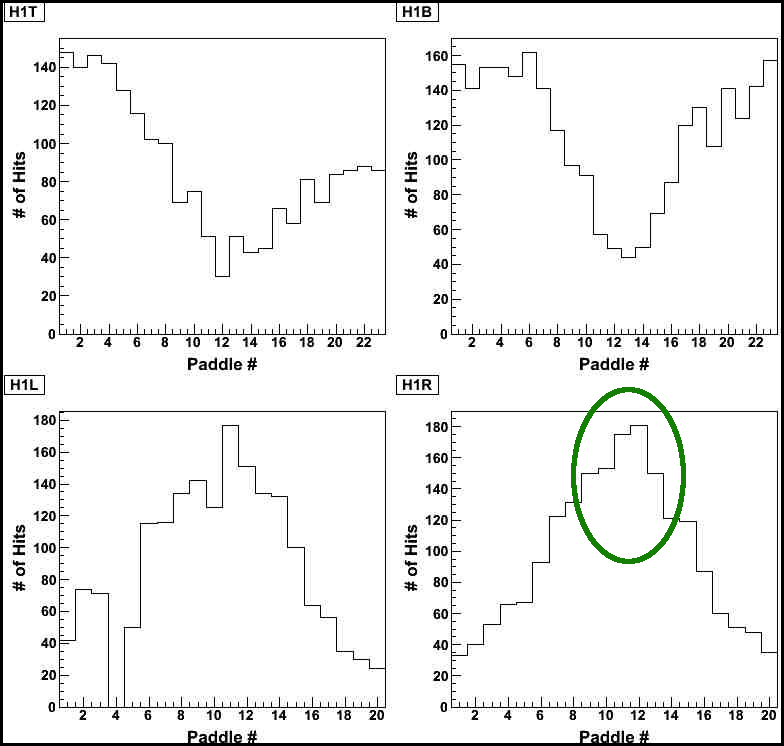
\includegraphics[width=0.5\textwidth]{figures/nosag.jpg} 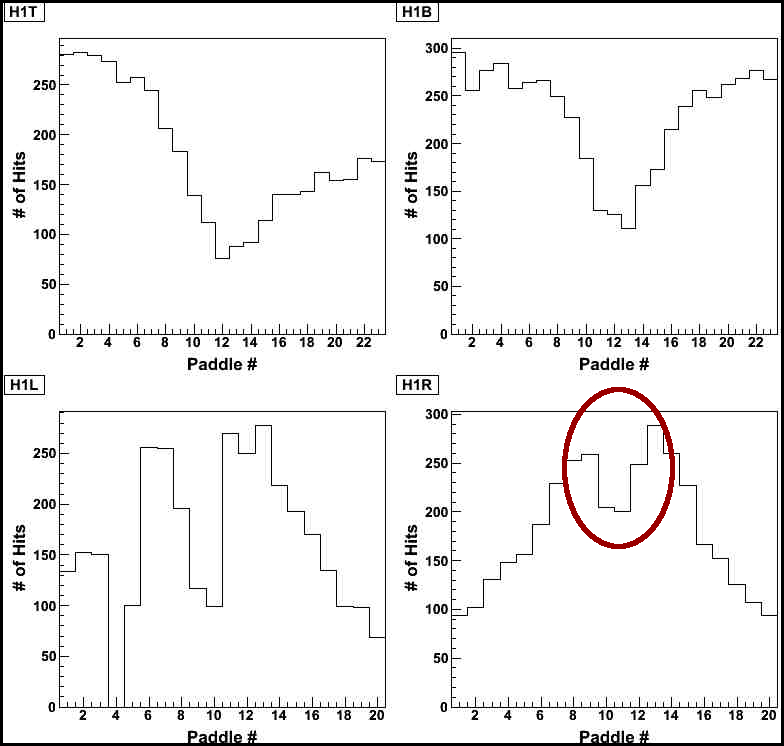
\includegraphics[width=0.5\textwidth]{figures/sag.jpg}}
	}
	\caption{(Left) Histogram of hodoscope `hits' in a typical event; (Right) Histogram of high-intensity event, with marked sagging most noticeably in the middle of the y-measuring hodoscopes}
	\label{fig:sag}
\end{figure}

During Run I of SeaQuest, observations of hodoscope wire maps (as in Fig.~\ref{fig:sag}) suggested an apparent drop in expected performance in the $y-$measuring hodoscopes. While this performance was most obviously seen in the $y-$measuring hodoscope planes, the $x-$measuring planes were likely also affected. This effect was assumed to be due to high-intensity RF buckets that caused very high multiplicity in all of the detectors in the spectrometer for that event. The result of these intense events seemed to push the PMTs and/or their PMT base electronics past their operational capacity.

The understood cause of this \emph{``sag''} in performance, as it came to be called, was due to a destabilization in the voltage divider in the PMT base. This critical component holds each dynode stage at a specific voltage, and when this destabilizes and is unable to maintain an appropriate voltage difference between dynode stages, inefficient performance of the PMT results.

During the Fall of 2012, prototyping and testing was performed with the goal in mind being to assemble a new base for the Philips XP-2008 PMTs~\cite{tubespecs} and compare its performance to the original PMT base and to some modern, high-performance Hamamatsu PMTs. Once a base design tested well, the new bases would be manufactured and installed in the existing frames of the original PMT bases.

\section{PMT Basic Construction and Operation}

\begin{figure}
	\centering
	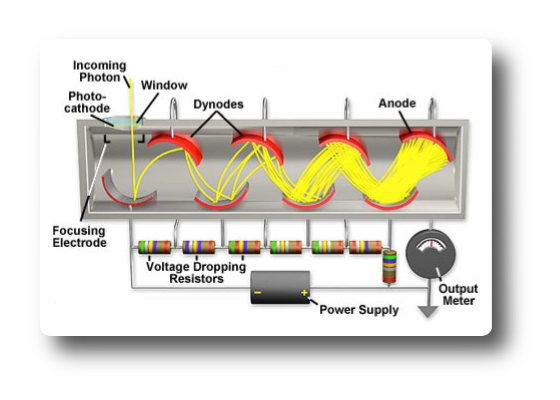
\includegraphics[width=0.5\textwidth]{figures/pmt-diagram.png}
	\caption{A diagram of typical PMT operation. The circuit controlling the voltage-dropping resistors is the part that was upgraded in this chapter.}
	\label{fig:pmt}
\end{figure}

Figure~\ref{fig:pmt} shows a schematic design of a typical photomultiplier tube and base setup. It consists of a photocathode that is followed by an electron multiplier section (or dynode string) then an anode from which a final signal is delivered. During operation, a high voltage is applied to the photocathode, dynodes, and anode in such a way that there's a potential ``ladder'' going from stage to stage. When an incident photon from the hodoscope scintillator paddle hits the photocathode, an electron is emitted via the photoelectric effect. The voltage difference between the cathode and dynode stages draws the emitted electron to the dynodes, and each time an electron hits a dynode, some of that electron's energy is transferred to other electrons in the dynode. These electrons then are emitted and become accelerated towards the next dynode stage. This process is called secondary emission, and by the time the process is repeated, there is a cascade or avalanche of electrons that land on the anode, resulting in a signal that can be amplified and analyzed.

It is the case that the voltage divider ultimately supplies the electrons that are emitted in this signal cascade. If too many photons and resultant electron cascades occur, the dynode stages' voltage divider will destabilize as they attempt to resupply the the dynode stages with electrons. The problem that was experienced at SeaQuest was that these high-intensity events were flooding the PMTs with photons, causing this ``saturation'' which caused this destabilization and the inefficient performance that was observed. The goal specifically was to test out modern base designs that provided for added stability to the performance of the voltage divider, even under high rates.

In general, each base divides around a \unit[-1500]{V} potential total over the photocathode (K), ten dynode stages (D1-D10), and the anode (A). There are two currents that are referred to here:
\begin{itemize}
	\item Signal Current: This is the signal that passes over the anode, which is the end-result of the cascading secondary emission electrons from each dynode stage.
	\item Bleeder Current: This is the current through the voltage divider. It is termed the ``bleeder'' current since the compounding electrons in the signal current must be ``bled'' from the current through the voltage divider.
\end{itemize}

Throughout these voltage base designs, capacitors are commonly implemented in the latter dynode stages where the most electrons are emitted. These capacitors, when charged, are able to replenish the lost charge on its corresponding dynode stage in the event that an intense light pulse induces a large signal current.  As the capacitor is able to hold its own charge, this resupply can occur without requiring the charges to be drawn from the bleeder current, thereby keeping the voltage across the dynode stages more stable.

\section{PMT Base Design Iterations}

There were several iterations of base design to determine which was best to approach for full base production and installation at SeaQuest. The core addition was the inclusion of transistors between dynode stages, according to the improvements suggested by C.R. Kerns in his paper regarding high-rate PMT bases~\cite{Kerns:1977qr}. Common solutions to destabilization in PMT bases have been to have (1) very large capacitor banks with charges $> 10^3$ times greater than the time-averaged dynode current and/or (2) miniature on-board,separately-powered Cockroft-Walton power supplies for the final dynode stages. A Kerns-style transistorized base allows for a light-weight, small size, and simple base that does not require extra power supplies or voluminous energy storage capacitors.

In general, there are three important features that were tuned in this set of prototypes that affected the performance of the phototubes:
\begin{itemize}
	\item
	Lower resistance
	\item
	Transistors (with protective diodes)
	\item
	Higher capacitance between dynode stages
	\item
	Distribution of voltage division
\end{itemize}

Lower overall resistance of the voltage divider increases the bleeder current. This means that the base will be more capable of handing high-intensity, as it will be better able to replenish the charges on each dynode stage in the case of a large signal. Typically, the larger the bleeder current, the larger the signal current can be without destabilizing the voltage divider. Higher rates usually put higher demand on the signal current, so by reducing the overall resistance, one can easily increase the rate capability. The shortfall here is that with voltage constant and resistance decreased, according to Ohm's Law ($V = IR$), the current will increase. As a result, the power dissipated by the circuit ($P = I^2 R$) will go as $I^2$, and the PMT base may heat up to critical temperatures faster than it can dissipate the heat as there is no significant ventilation in the PMT base enclosure. The Philips XP-2008 manual quotes that for continuous usage and storage the ambient temperature should not exceed $50^\circ C$ ($122^\circ F$). In addition to heat concerns, there's typically a power rating for the class of small on-board resistors that were planned to be used. Approaching or exceeding that power limit would run the risk of burning out a resistor and rendering the base inoperable. 

\begin{figure}
	\centering
	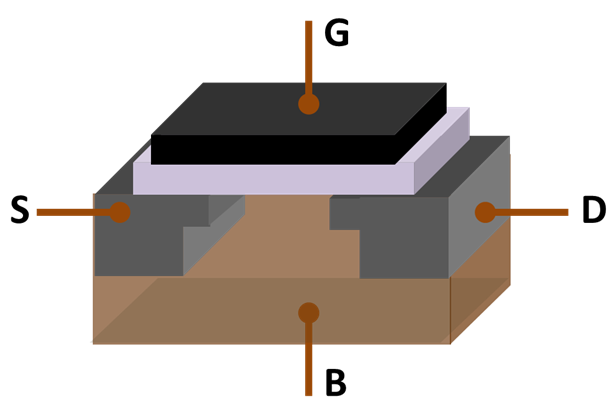
\includegraphics[width=0.5\textwidth]{figures/MOSFET_Structure.png}
	\caption{MOSFET showing gate (G), body (B), source (S) and drain (D) terminals. The gate is separated from the body by an insulating layer (white)~\cite{wmc:mosfet}}
	\label{fig:mosfet}
\end{figure}

Metal–oxide–semiconductor field-effect transistors (MOSFETs) are introduced here to maintain the proper voltage division. In general, MOSFET transistors have an \emph{source}, a \emph{drain}, and a \emph{gate}, where current flows freely through from the source to the drain, gate permitting. If at any point a certain voltage across the gate of the transistor is not supplied (here, the voltage across dynode stages), then the source-to-drain current through the transistor is stopped until the proper gate voltage is restored. This helps greatly to ``intelligently'' regulate the voltage across the dynodes. Wherever transistors are used, diodes are also implemented to prevent the unlikely case of a current moving across the transistors' gate in the wrong direction. This protects the transistors from being damaged particularly when powering the circuit on and off.

Having capacitors along the higher dynode stages allows for quick resupply of charges to the dynodes, thus maintaining proper voltage division. This, however, is only a stop-gap measure and is only effective under cases of high instantaneous currents. It is the case that, should there be a constant too-high rate of operation, the capacitors will not be able to recharge themselves. Typical recharge time for the capacitors discussed in this section can range from \unit[0.1-1]{ms}.

Finally, the specific division of voltage across each stage, from D1 to A, has an influence on the behavior of the PMT operation. As we see from the operations manual of the phototube in Fig.~\ref{fig:voltage_schemes}, in the case of a progressively increasing voltage division, there is a good compromise between timing and linearity. With respect to phototube operation, ``linearity'' is the quality that the amount of charge deposited on the anode is linearly proportional to the energy of the incident photon. ``Timing'', on the other hand, is the quality that the time it takes for a high-energy photon signal and a low-energy photon signal to progress through the stages should be the same. For the purpose of optimization at SeaQuest, we wish to optimize the amount of signal (i.e. amplification or \emph{gain}) that the phototube can accommodate. For this, the recommended voltage partitioning is flat from D1-A~\cite{tubespecs}.

It should be noted that the prototype iterations of PMT base design changes was not intended to cover the entire phase space of these tunable parameters. The purpose of these tests were to get a sense of how changing one or more of these parameters could affect the PMT high-rate capabilities. The decision for a final base design had to be decided on with relative speed to get them manufactured, built, and installed before Run II of the experiment. As such, true optimization of all parameters could not be achieved within the scope of these tests.

\begin{figure}
	\centering
	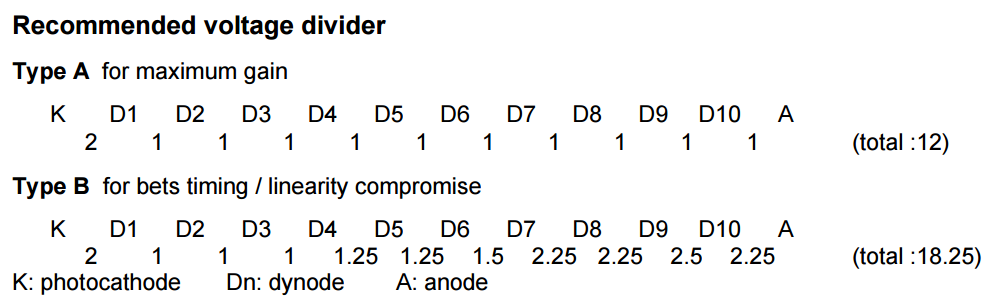
\includegraphics[width=0.7\textwidth]{figures/voltage_divider.png}
	\caption{Suggested voltage division schemes for gain vs. timing/linearity compromise~\cite{tubespecs}.}
	\label{fig:voltage_schemes}
\end{figure}

\subsection{Original Base}

The base that came attached to the PMTs were manufactured specifically for use by the ARGUS experiment, which was a relatively (by SeaQuest standards) lower-rate collider experiment that used $e^+ e^-$ annihilation at the \emph{DORIS\ II} ring at DESY. After their tenure at ARGUS, they were handed down to the HERMES experiment located at the \emph{HERA} polarized electron accelerator at DESY.

Though no actual circuit diagram was documented for the original PMT base, it was dissected and each component was measured. The results can be found in Fig.~\ref{fig:original-board}, and its voltage division seen in Fig.~\ref{fig:original-volt}. It features a simple string of resistors with capacitors of increasing capacitance along the last six stages. The voltage division can be recognized to be similar to the timing-linearity compromise scheme described in Fig.~\ref{fig:voltage_schemes}. With a total resistance of approximately \unit[3.95]{$M\Omega$} and the operational voltage of \unit[-1500]{V}, the expected standing (bleeder) current even when sitting in the dark is expected to be \unit[0.38]{mA}. With this in mind, we would expect the voltage divider to destabilize when the signal current approaches this value.

\begin{figure}
	\centerline{
		\mbox{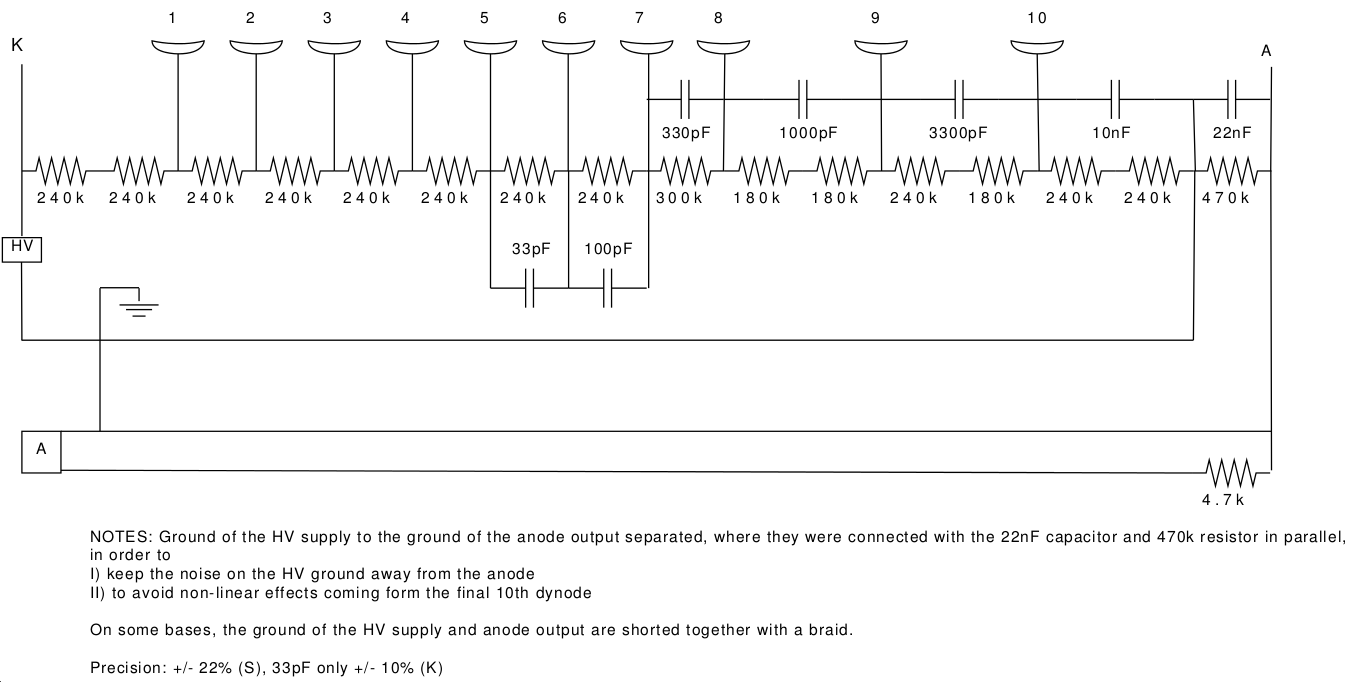
\includegraphics[width=0.75\textwidth]{figures/pmt.png}}
	}
	\caption{The original PMT base inherited from the ARGUS and HERMES experiments.}
	\label{fig:original-board}
\end{figure}

\begin{figure}
	\centerline{
		\mbox{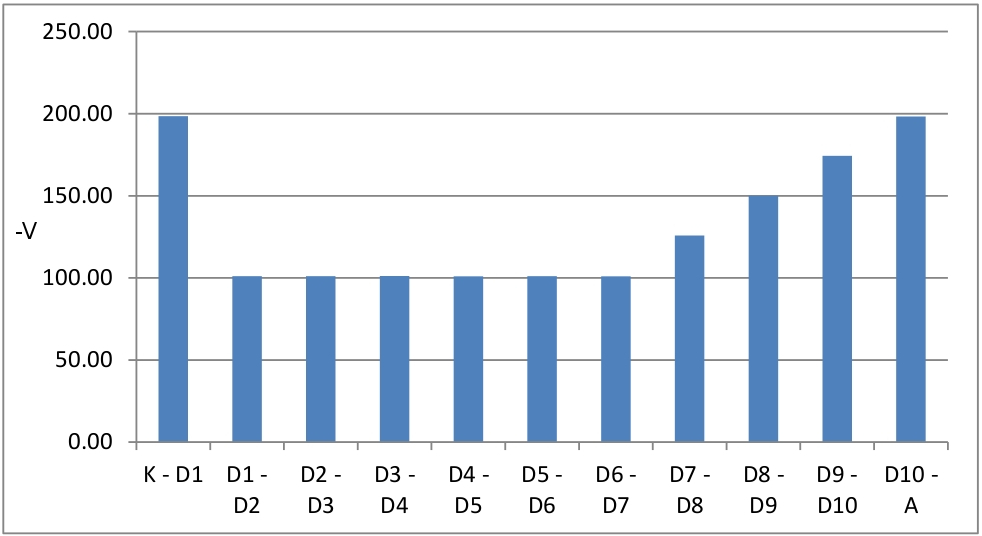
\includegraphics[width=0.55\textwidth]{figures/original-volt.jpg}}
	}
	\caption{The voltage division between subsequent stages for the original PMT base design when supplied with \unit[-1500]{V}.}
	\label{fig:original-volt}
\end{figure}

\subsection{Prototype Base v1}

Once the task was set to update the PMT base design, the Fermilab Particle Physics Division was consulted on the matter. In 2010 a base design with similar goals for the exact same PMT model was designed by Sten Hansen~\cite{pc:sten}. The circuit diagram for the new base can be found in Fig.~\ref{fig:v1-board}.

Here, the resistance was significantly reduced by a factor of about 2.9, allowing for much more bleeder current, without exceeding or closely approaching the on-board resistors' power rating. Also, the voltage division was designed to be relatively ``flat'' (Fig.~\ref{fig:v123-volt}) across stages from D1 to A, which is stated to be recommended for optimal gain. With a total resistance of approximately \unit[1365]{$k\Omega$} and the operational voltage of \unit[-1500]{V}, the expected standing (bleeder) current even when sitting in the dark is expected to be \unit[1.1]{mA}. Already here, we see that this design parameter alone suggests its ability to withstand $\sim 3x$ more signal current as compared to the original base.

The introduction of MOSFET transistors is seen between each stage from D7 to D10. Sending the current in parallel over a \unit[1]{$M\Omega$} resistors allows the gate of the transistor to measure the voltage without drawing much current. The Zener dynodes are there in place before each transistor gate to ensure that current only goes one way across the sensitive gate channels.

It is also notable that there are banks of capacitors in parallel across the higher dynode stages. Since there is higher current through this circuit than the original base under the same voltage, there will be greater demand on the capacitors to resupply the dynode stages with spent charge. The two \unit[10]{nF} capacitors in parallel across each stage (which amount to \unit[20]{nF} total) is significantly greater than the capacitance across the stages of the original base.

\begin{figure}
	\centerline{
		\mbox{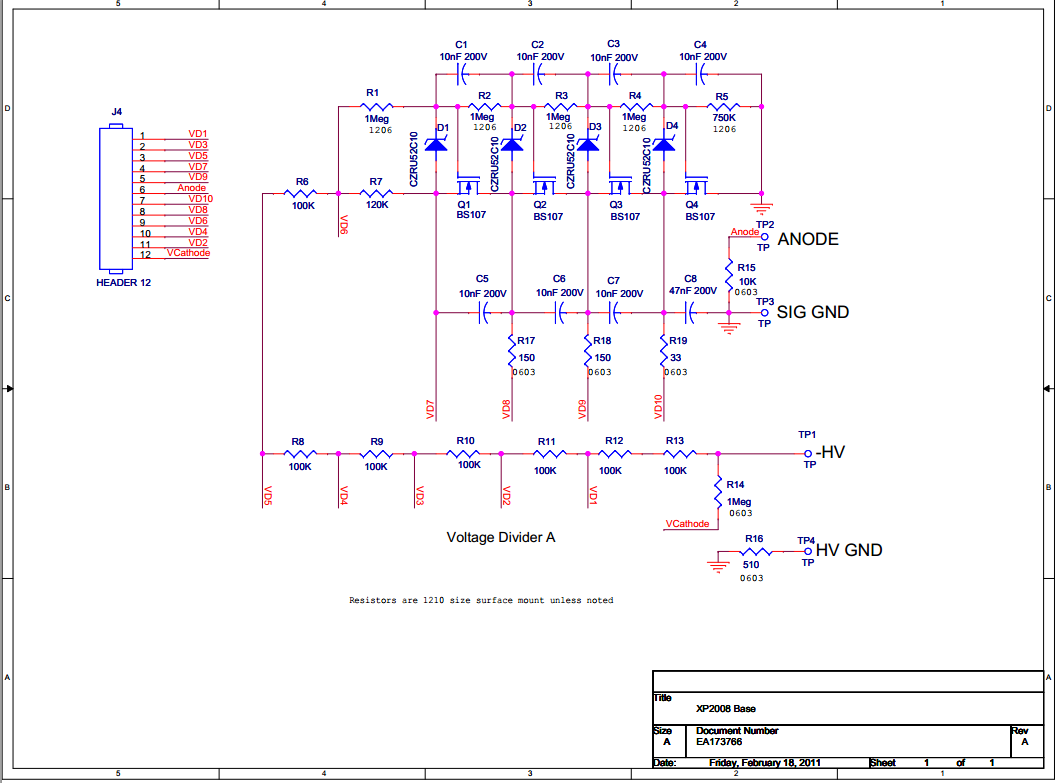
\includegraphics[width=0.7\textwidth]{figures/newbase.png}}
	}
	\caption{The Prototype v1 board circuit diagram received from Fermilab Particle Physics Division~\cite{pc:sten}. The parts are denoted as R: resistor, C: capacitor, Q: MOSFET transistor, D: Zener diode.}
	\label{fig:v1-board}
\end{figure}

\begin{figure}
	\centerline{
		\mbox{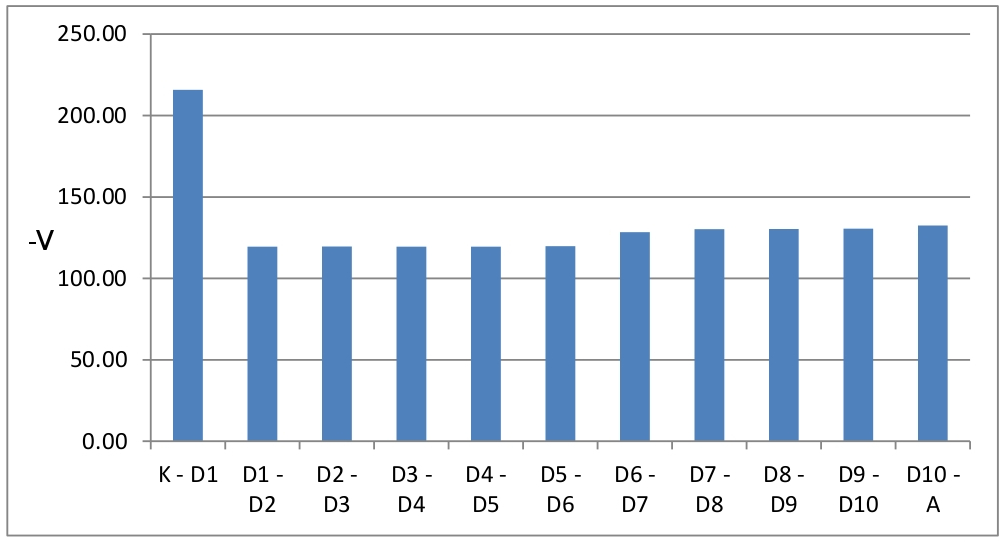
\includegraphics[width=0.55\textwidth]{figures/v123-volt.jpg}}
	}
	\caption{The voltage devision between subsequent stages for the Prototypes v1, v2, and v3 PMT base designs  when supplied with \unit[-1500]{V}.}
	\label{fig:v123-volt}
\end{figure}

\subsection{Prototype Base v2}

The first modification made to the prototype board was to keep everything identical except for the total resistance of the circuit. This was accomplished by halving the resistance of each of the first six stages (R6-R13 on Fig.~\ref{fig:v1-board}) from to increase the bleeder current. The resulting current of the base at \unit[-1500]{V} is at around \unit[2.2]{mA}. The voltage division retained the same values as described in Fig.~\ref{fig:v123-volt}.

\subsection{Prototype Base v3}

In the case that destabilization was occurring prior to the dynode stages with the added capacitors and transistors, the third prototype was decided to take the Prototype v1 design and add more ``transistorized'' stages earlier on. This entailed extending the parallel configuration of capacitors, transistor, diode, and \unit[1]{$M\Omega$} to the D5-D6 and D6-D7 stages. This prototype configuration can be seen in Fig.~\ref{fig:v3-board}). The voltage division was not significantly altered by this change and remained relatively the same as what is described in Fig.~\ref{fig:v123-volt}.

\begin{figure}
	\centerline{
		\mbox{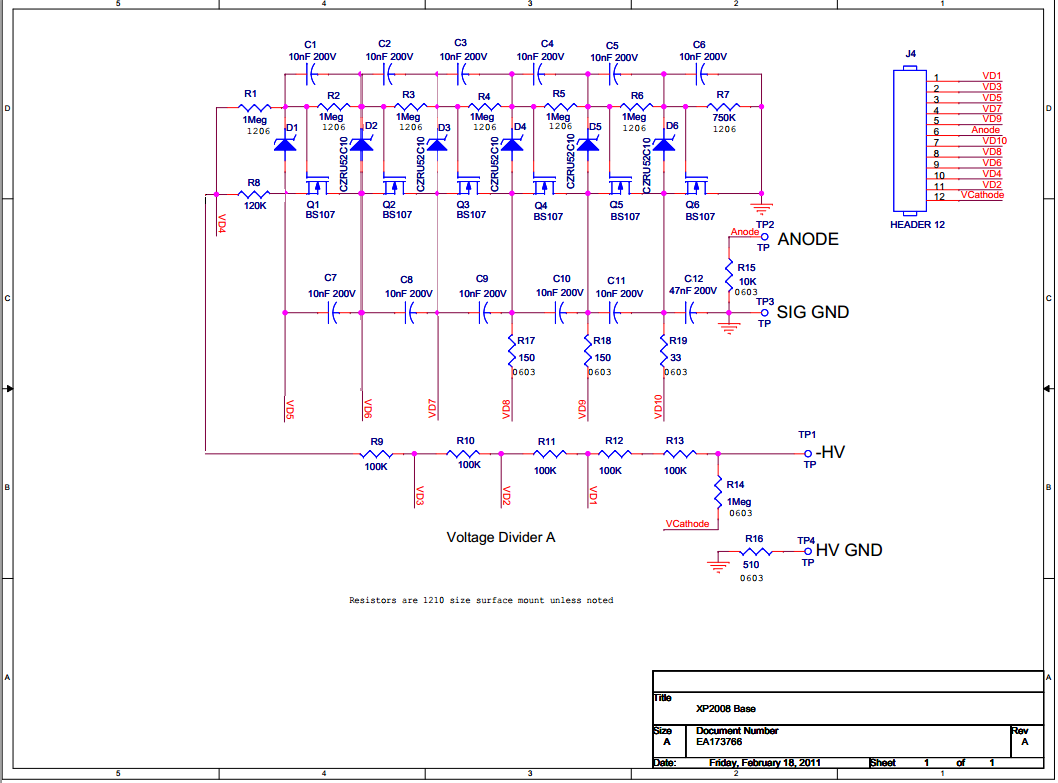
\includegraphics[width=0.7\textwidth]{figures/newbase_6mosfet.png}}
	}
	\caption{The Prototype v3 board: 3 more transistorized stages than the Prototype v1 design.}
	\label{fig:v3-board}
\end{figure}

\subsection{Prototype Base v4}

The final modification arose from a suggestion from a Fermilab collaborator. It was suggested that it may significantly extend the dynamic range of the tube/base by increasing the voltage drop in, specifically, the last stage relative to the other stages.  This reduced to simply replacing R5 (of Fig.~\ref{fig:v1-board}), a \unit[1]{$M\Omega$} resistor, with a \unit[1.5]{$M\Omega$}.  All of the rest would remain unchanged from Prototype v1. The premise for this modification was in the case that the final batch of electrons needed help being ``swept'' to the anode with a higher voltage difference. The change applied resulted in the voltage distribution accorging to Fig.~\ref{fig:v4-volt}.

\begin{figure}
	\centerline{
		\mbox{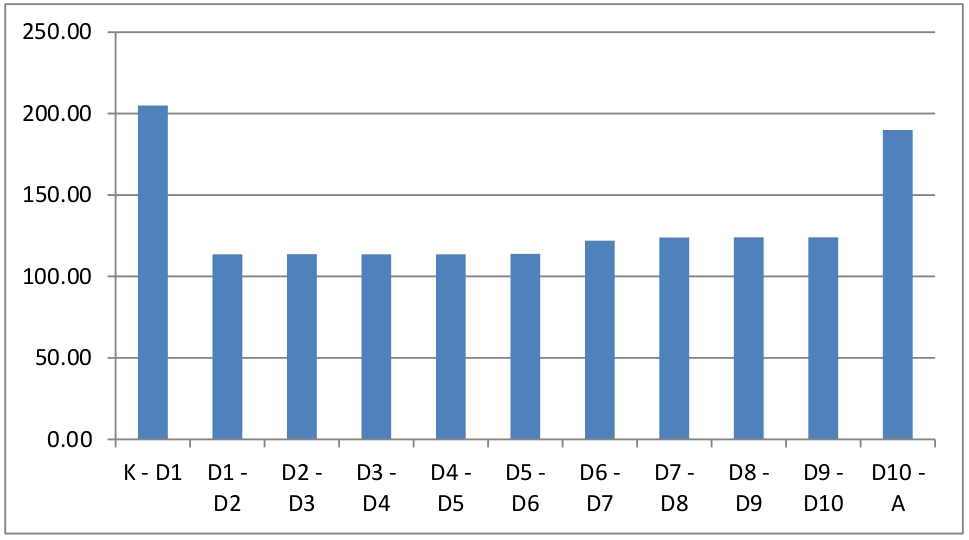
\includegraphics[width=0.55\textwidth]{figures/v4-volt.jpg}}
	}
	\caption{The (negative) voltage between subsequent stages for the Prototype v4 PMT base.}
	\label{fig:v4-volt}
\end{figure}

\section{PMT Base Comparisons}

There is a specific difficulty with the objective to increase the rate capability of our PMT's. This difficulty is that there was not a known instantaneous intensity or target rate capability to attain. The rate and intensity that caused the original PMT performance to sag is unknown, and if it was known, it would be difficult to match the intensity with an experimental setup. As a result, the objective in these tests was to \emph{compare} the performance of the same PMT under controlled conditions using the original and various prototype bases.

Due to the effects of using different PMTs and due to temperature and humidity fluctuations, the PMT behavior can be somewhat variable from test to test. For this reason, one can only reasonably compare results within each base comparison test, and not across different comparison tests. Each was performed on different days, and sometimes with different PMT’s.

\subsection{Testing Apparatus, Measurements, and Procedure}

In this experiment, a PMT attached to a PMT base was placed into a light-tight box facing a fast-pulsing 470nm wavelength LED, which provides the driving photonic signal. 

\subsubsection{PMT Test Setup}

The LED light source assembly consisted of a machined aluminum block that housed the LED, which was a fast-pulsing, narrow beam, water-clear blue LED, peaking in the $\lambda =$\unit[450]{nm} region. This block had a sliding aluminum insert which had a $1/4$'' depression used for inserting a 1'' diameter NDF of arbitrary optical density~\cite{ames1998measurement}. The LED, according to specifications, has a \unit[N]{ns} rise time and a \unit[N]{ns} fall time, which is important when considering pulsing frequencies on the order of \unit[30]{MHz}.

The LED itself was driven by an Agilent 33520 Function / Arbitrary Waveform Generator~\cite{agilent:33520} capable of generating signals up to 30MHz. The LED's unadulterated intensity was by far too much light to perform any useful test with such photosensitive hardware. Its intensity was attenuated by use of a neutral density filter (NDF), with a rating $D=3.0$, where the NDF allows 1 in $10^D$ photons through (1 in 1000 for $D=3.0$). When testing began, a $D=4.0$ NDF was used, but the amount of light reaching the PMT was so small that no decrease in PMT performance for any of the bases was observed all the way up to the highest LED frequencies. As such, the $D=3.0$ NDF was chosed for this study.

These were all kept within the light-tight box\footnote{These light-tight boxes are paradoxically referred to as both ``light boxes'' and ``dark boxes'', as they're used for testing \emph{light}-sensitive equipment and they're made to be very \emph{dark} inside.} loaned to the SeaQuest collaboration from the Daya Bay group. This light box was equipped with a patch panel that had both BNC and HVBNC connectors by which to power the PMT base and read out its signal. The light box and all of the installed components can be seen in Fig.~\ref{fig:pmtsetup}.

\begin{figure}
	\centerline{
		\mbox{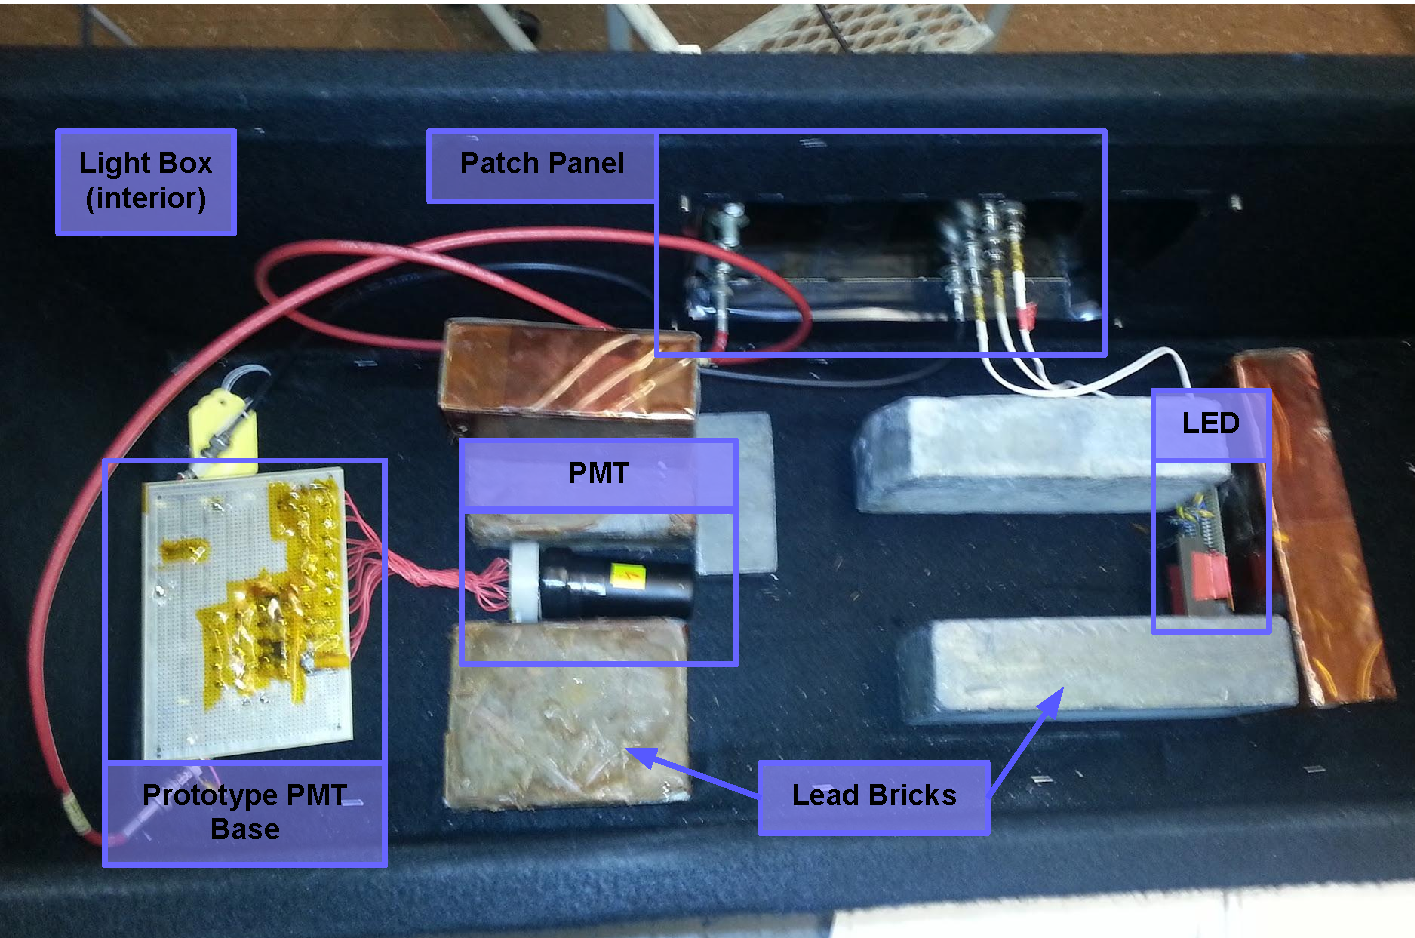
\includegraphics[width=0.75\textwidth]{figures/LightBox.pdf}}
	}
	\caption{Inside of the light box, with the prototype board (left) wired up to a Philips XP-2008 PMT (middle), facing a fast-pulsing LED source (right).}
	\label{fig:pmtsetup}
\end{figure}

A simple data acquisition was assembled from an amplifier, discriminator, and scaler in order to observe that the PMT was functioning properly and firing off at the rate that the LED was set to pulse at.

\subsubsection{Measured and Calculated Quantities}

The PMT base was powered by a high voltage supply, and an ammeter was connected between the two in order to measure the amount of current drawn, or bleeder current, from the HV power supply. The PMT signal was processed by an oscilloscope, averaging the pulse over 300 pulses. The primary measurement was measuring the area of the averaged pulse ($V\cdot s$).

We calculated the signal current from the anode as:
\begin{eqnarray}
	Q_{pulse} & = & \frac{\int V dt}{R} \\
	I_{signal} & = & f Q_{pulse}
\end{eqnarray}
where $f$ here is the driving frequency of the pulsing LED, $R$ is the termination resistance of the signal (\unit[50]{$\Omega$}), and $\int V dt$ is the integrated area of the averaged PMT pulse. The amplitude of the pulses was also measured, as it was important in determining if it were feasible to remove the typically noisy hodoscope amplifiers from the SeaQuest stations 1 and 2 DAQ setup.

The measured and calculated quantities of interest are the bleeder current, the averaged signal amplitude, averaged signal area, and signal current over the anode.

Due to the limitations of the instruments used in these tests, there is some systematic uncertainty to consider. The ammeter used to measure the bleeder current between the HV supply and the PMT base used an analog gauge that had closely spaced ticks at \unit[0.2]{mA} intervals. As such, the systematic uncertainty for the bleeder current is considered to be $\pm$\unit[0.05]{mA}. Also, due to pulse-to-pulse variations which cause a mild amount of smearing in the average, the measurement of the amplitudes and signal areas have an uncertainty of $\pm$\unit[5]{mV} and $\pm$\unit[0.1]{nVs}, respectively. The uncertainty in the signal area translates to an uncertainty in the calculated signal current of around $\pm$\unit[0.04]{mA}. These fluctuations are considered negligible with respect to the quantities measured.

\subsubsection{Test Procedure}

Most of the prototyping was performed over the span of two weeks. As new suggestions were made at base improvements and the iterations v1-v4 progressed, more comparison tests were performed. The procedure for the each test was the same and is as follows:
\begin{enumerate}[itemsep=-1ex]
	\item Connect the base to the PMT and to the HVBNC and BNC connectors.
	\item Close the lid to the light box.
	\item Gradually power the PMT (\unit[-250]{V} every \unit[5]{s}) until it is as \unit[-1500]{V}.
	\item Watch the scaler on the DAQ to see if it is rapidly counting. No (or very few) counts on the scaler. means the box is light-tight.
	\item Let the PMT and base warm up to near-operational temperatures with its standing current for a minute or two.
	\item Power on the function generator and LED, setting the function generator to create a \unit[16]{ns} square wave pulse to the LED circuit (the minimum achievable pulse width~\cite{agilent:33520}) at a frequency of \unit[10]{Hz}.
	\item For each of several frequencies from \unit[10]{Hz} to \unit[30]{MHz}, perform the following:
	\begin{enumerate}[itemsep=-1ex]
		\item Observe the scaler to ensure that the count is increasing at the same rate as is set by the function generator. This confirms that both the PMT, base, function generator, and LED are generally working as planned.
		\item Trigger on the signal from the PMT output.
		\item Average the signal over 300 triggered pulses and then freeze the frame.
		\item Record the current draw from the HV supply (bleeder current).
		\item Measure and record the pulse amplitude with the oscilloscope cursor.
		\item Measure the pulse area using the signal integration feature, setting vertical cursors at the zero-intercept on each side of the pulse.
		\item Return to triggering mode and increase the function generator frequency as warranted.
	\end{enumerate}
	\item Power off the function generator and LED circuit.
	\item Step the PMT voltage down slowly to \unit[0]{V}.
	\item Open the light box and replace the base for subsequent tests as necessary, repeating the steps above.
\end{enumerate}

\subsection{Original vs. Prototype v1}

The first test was to compare the original base with the first iteration of the prototype base. It was generally expected that this new design with more modern technology would exceed the performance of the original base, but the question was twofold: to what extent does it perform better and what is the baseline by which to compare future improvements? 

\begin{figure}[ht]
	\centerline{
		\mbox{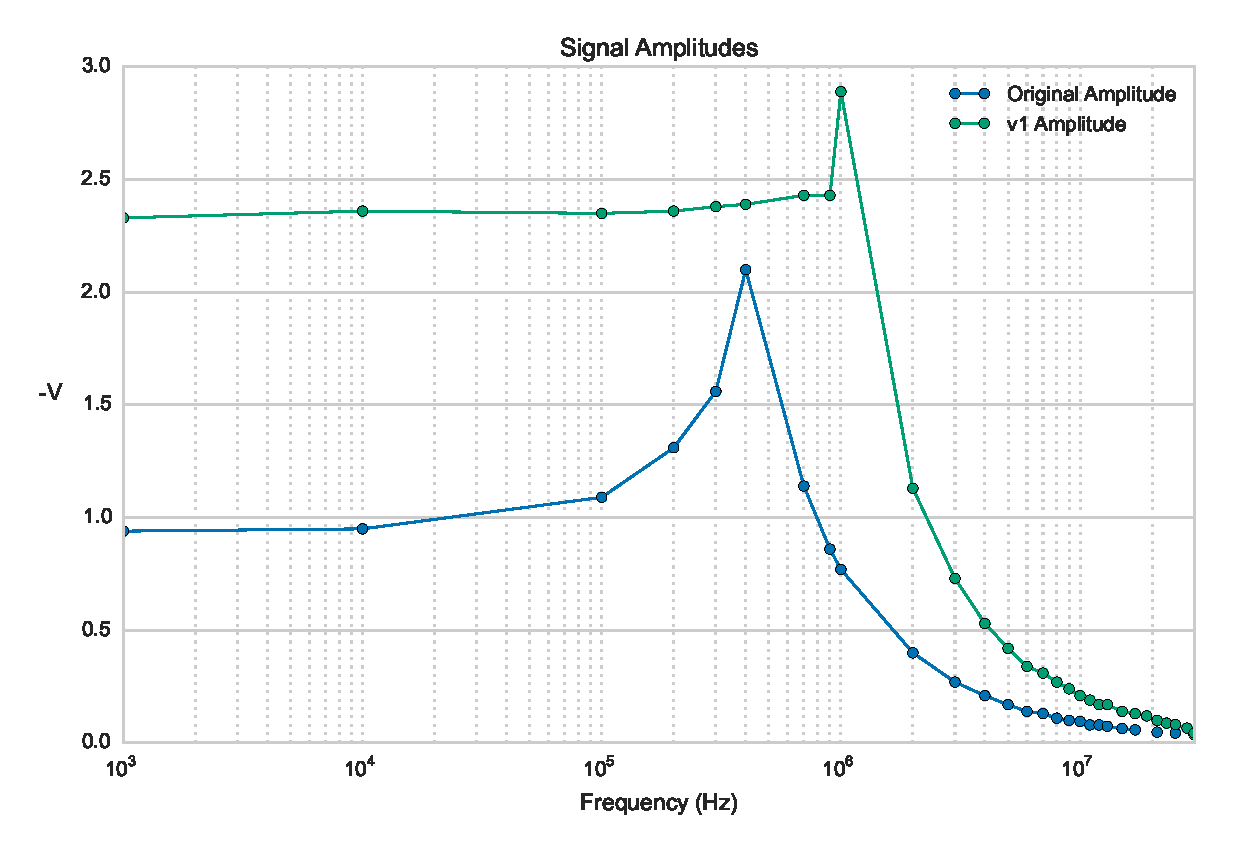
\includegraphics[width=0.5\textwidth]{figures/Test_v1_Amp.eps} 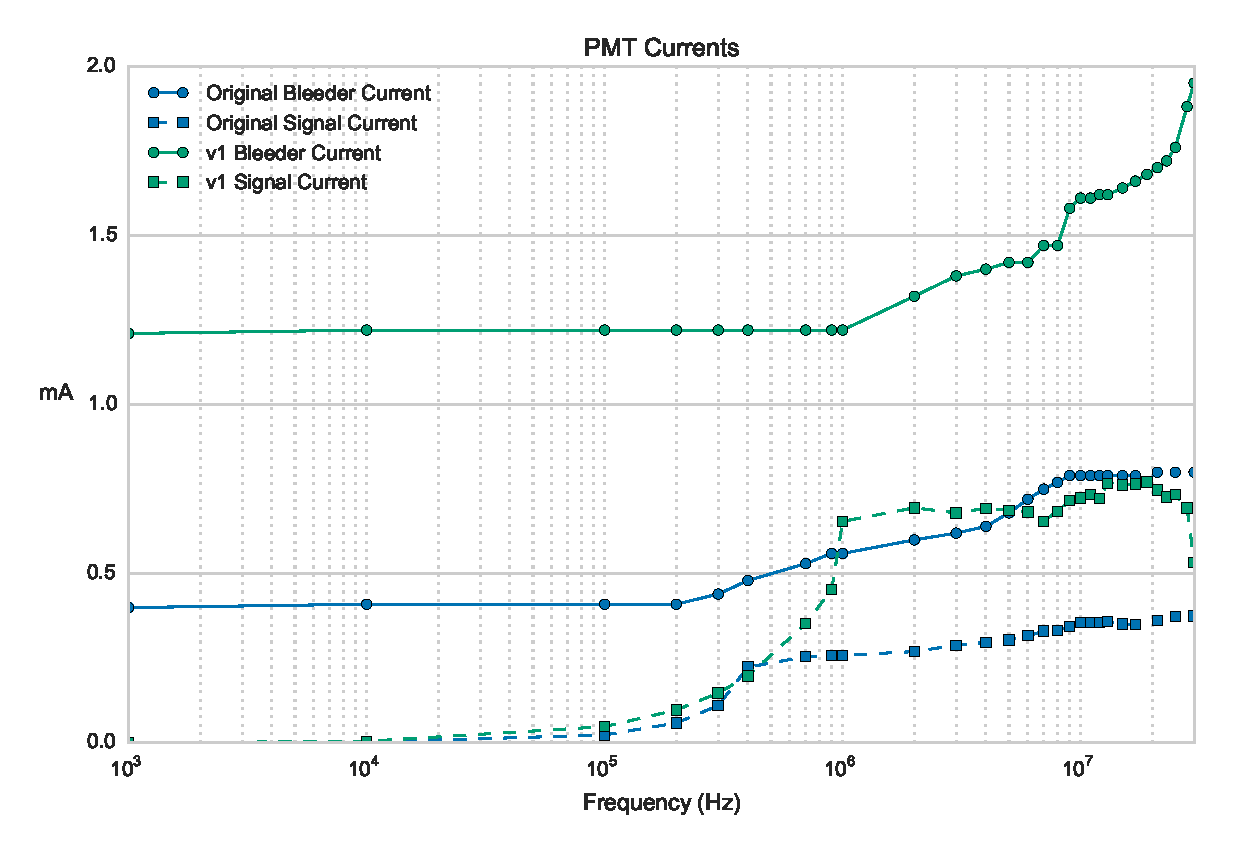
\includegraphics[width=0.5\textwidth]{figures/Test_v1_Current.eps}}}
	\caption{Measurements of the (a) signal amplitudes and (b) bleeder and signal currents in the original and prototype v1 PMT bases. The HV was inadvertently set to \unit[-1600V]{V} for this test instead of the intended \unit[-1500]{V}.}
	\label{fig:test-v1}
\end{figure}

The first important observation is the baseline amplitudes of the signals from the two bases, as seen in Fig.~\ref{fig:test-v1}(a). While the absolute voltage itself is not as useful since the LED doesn't necessarily reflect actual operating conditions, we do see that the amplitude from the new base design is increased by a factor of more than two. This in itself is significant in when considering the limits of the discriminators that were used in the hodoscope arrays for Stations 1 and 2. With even a modest boost to gain and signal amplitude, the PMT signals should be large enough that an amplifier is not required in order to get a discriminator to trigger on a PMT pulse. Seeing as the amplifiers used had often caused troubles with the amount of electronic noise they tended to imbue, this was an encouraging observation.

Next, we look at the behavior of the amplitudes as the frequency progresses. It is safe to assume that the unchanging behavior in the lower frequencies indicate that the voltage divider is stable and that there is no voltage break down yet. At higher frequencies, there is a qualitative peak in amplitude for both bases, followed by a steep decline. This rise and then sharp fall would seem to indicate the end of stable PMT base operation, with the fall indicating the onset of degradation of performance.

To better identify the conditions that cause this onset, we look to currents applicable to both bases (Fig.~\ref{fig:test-v1}(b)). In this particular test, we see the original base peak in amplitude at $\sim$\unit[4]{MHz} and prototype base v1 peak at $\sim$\unit[10]{MHz}. Looking to the currents, we see that these particular points mark a certain point for both where the signal current reaches almost exactly 50\% of the bleeder current. The baseline improvement with this base over the original one was estimated to extend the operational range by a factor of three -- the point where the amplitude drops below the low-frequency baseline.

Around the time of these tests, Sten Hansen conducted a SPICE (Simulation Program with Integrated Circuit Emphasis) simulation of the prototype circuit and was able to reproduce what was observed. In particular, it was observed that the gain began to change dramatically when the anode (signal) current reaches a significant fraction of the total current drawn from the HV supply; a current that is much less than 100\%. It was concluded that 50\% was consistent with his findings.

\subsection{Original vs. Prototype v1 vs. Prototype v2}

Several suggestions were made in altering the prototype base in order to maximize this improvement, including lowering the overall resistance of the circuit. If the signal current grows at the same pace, then by increasing the bleeder current, there is a chance that a higher frequency signal will be required to bring the signal current up to the point where the divider breaks down, which we estimated above to be $\sim 50\%$ of the increased bleeder current.

\begin{figure}[h]
	\centerline{
		\mbox{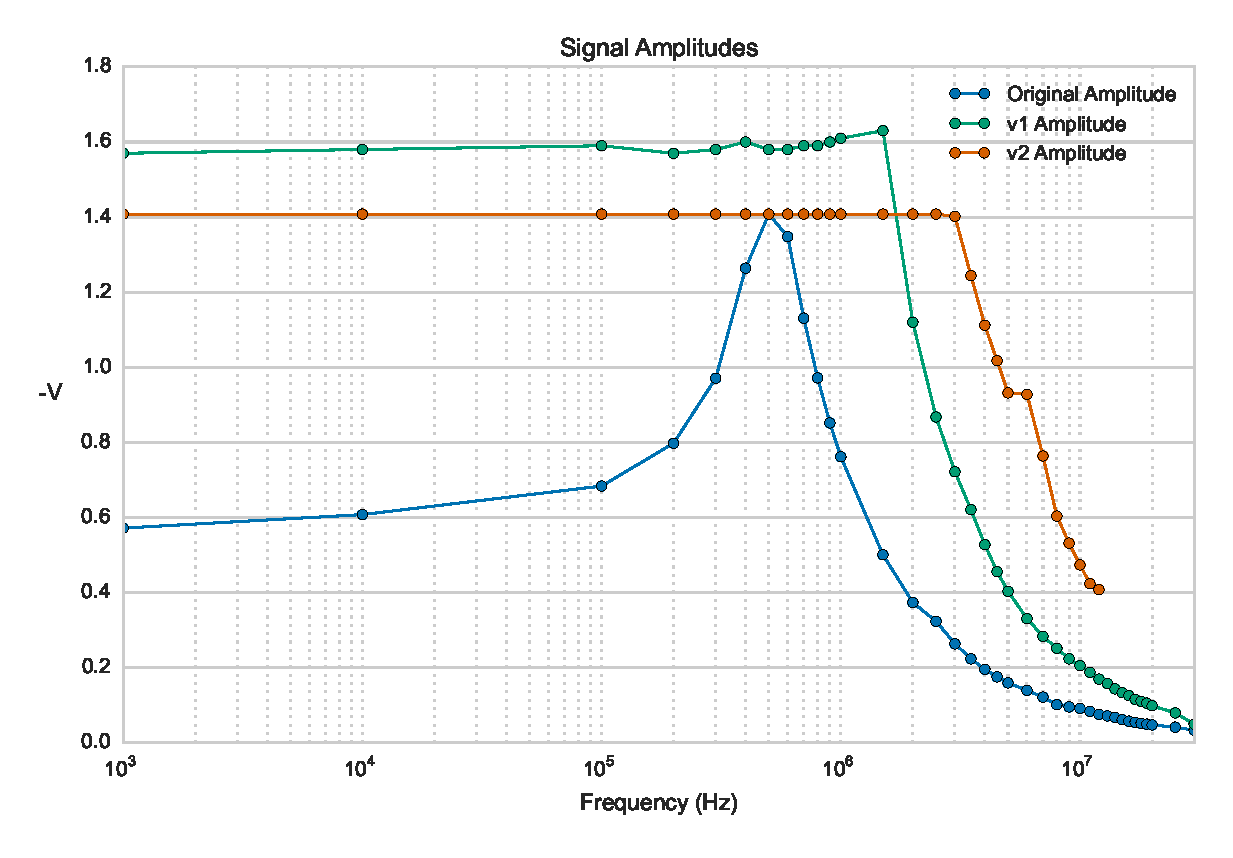
\includegraphics[width=0.5\textwidth]{figures/Test_v2_Amp.eps} 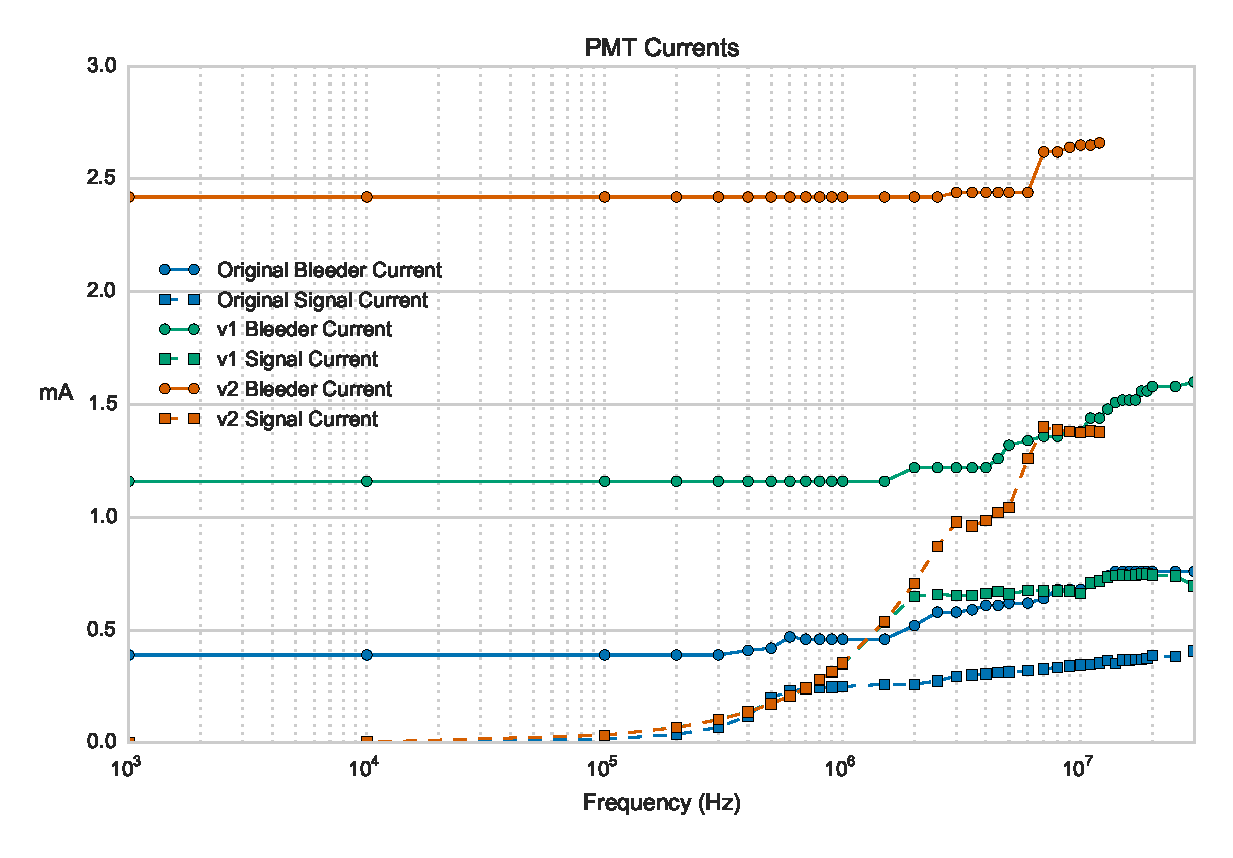
\includegraphics[width=0.5\textwidth]{figures/Test_v2_Current.eps}}}
	\caption{Measurements of the (a) signal amplitudes and (b) bleeder and signal currents in the original, prototype v1, and prototype v2 PMT bases.}
	\label{fig:test-v2}
\end{figure}

Looking to Figure~\ref{fig:test-v2}(a), we see that this basic premise is technically sound. The prototype v2 base exceeds the dynamic range of both the original base and the prototype v1 base by factors of approximately a factor of four and two, respectively. This is a a significant improvement, and this at first seems to be an avenue to pursue. However, an issue arose after increasing the LED frequency from \unit[13]{MHz} to \unit[14]{MHz} when a resistor burned out. The test continued with the rest of the bases, but the results paint a clear picture of what happened. 

By halving the resistance, the bleeder current doubled (Figure~\ref{fig:test-v2}(b)). This caused the power being dissipated by the resistors to exceed their power rating. The prototype bases were built with \unit[0.25]{W} resistors, and as the bleeder current rose well above \unit[2.5]{mA}, one of the resistors failed. This did not bode well for how a smaller on-board resistor might fare with the same current.

To further exacerbate matters, it was found that our LeCroy 1440 HV supplies could only supply a maximum of \unit[2.5]{mA} per channel~\cite{lecroy:1440}. Seeing as these power supplies had proven themselves sensitive and prone to communication and performance failures, it was deemed inadvisable to demand anywhere near the maximum current from these HV supplies.

For these reasons, it was decided that the new PMT base design of prototype v1 not be modified in this manner which might suffer from overheating, component failure, and a too-high current demand.

\subsection{Prototype v1 vs. Prototype v3}

Perhaps it was the case that the ``transistorized'' steps were doing their job well and the destabilization was occurring at prior stages. Since the only downside of adding additional steps was added cost, transistorized stages were added as depicted in Fig.~\ref{fig:v3-board}.

\begin{figure}[h]
	\centerline{
		\mbox{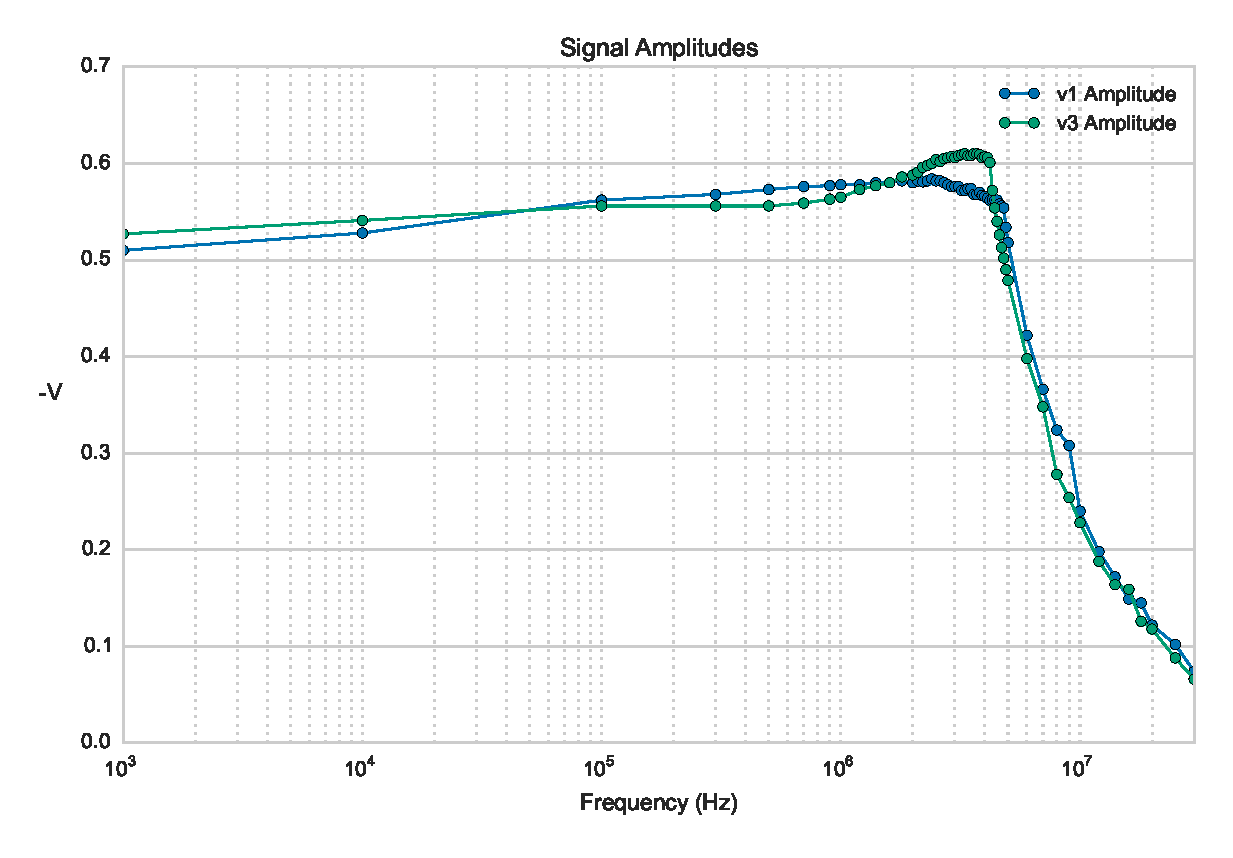
\includegraphics[width=0.5\textwidth]{figures/Test_v3_Amp.eps} 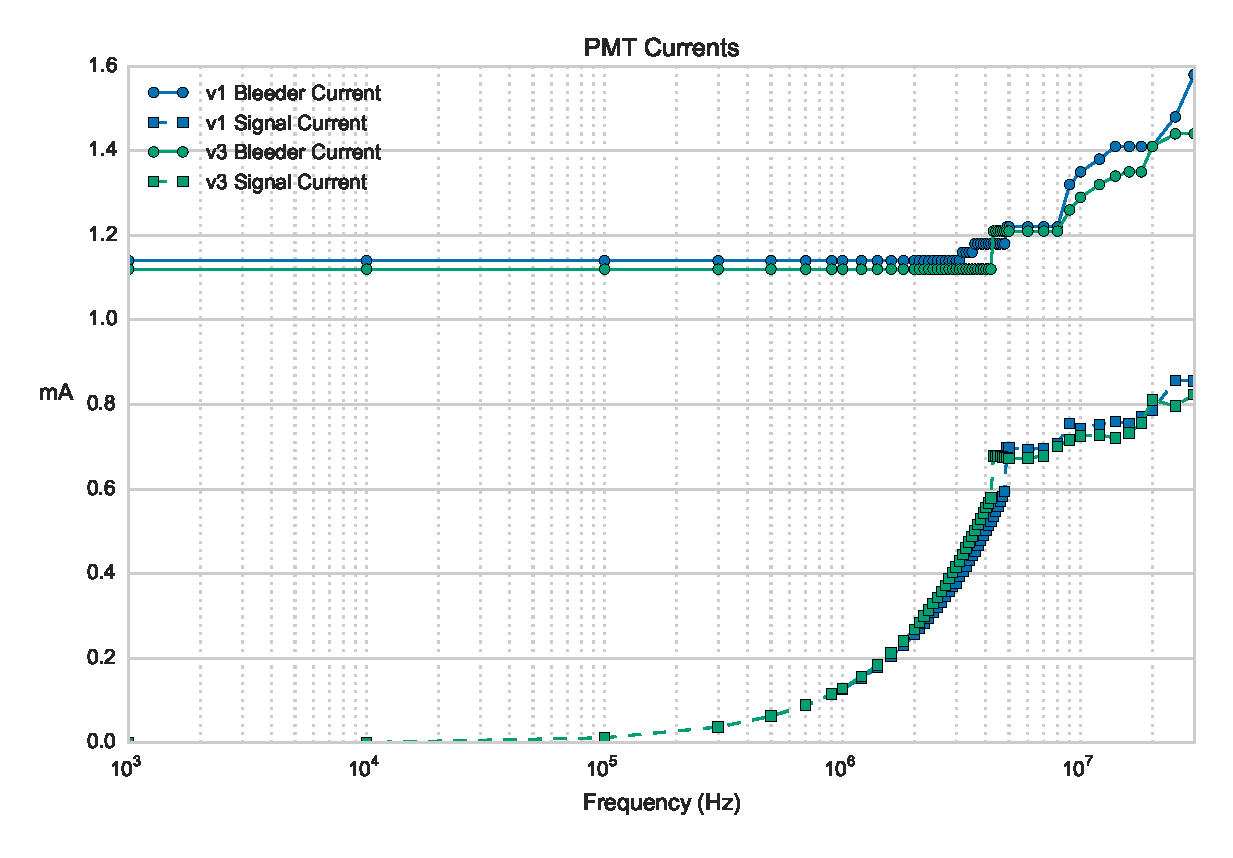
\includegraphics[width=0.5\textwidth]{figures/Test_v3_Current.eps}}}
	\caption{Measurements of the (a) signal amplitudes and (b) bleeder and signal currents in the prototype v1 and prototype v3 PMT bases.}
	\label{fig:test-v3}
\end{figure}

As is quite evident in Figure~\ref{fig:test-v3}, there was no significant difference in the performance of the two prototype bases. As such, this modification was not adopted into the final design.

\subsection{Prototype v1 vs. Prototype v4}



\begin{figure}[h]
	\centerline{
		\mbox{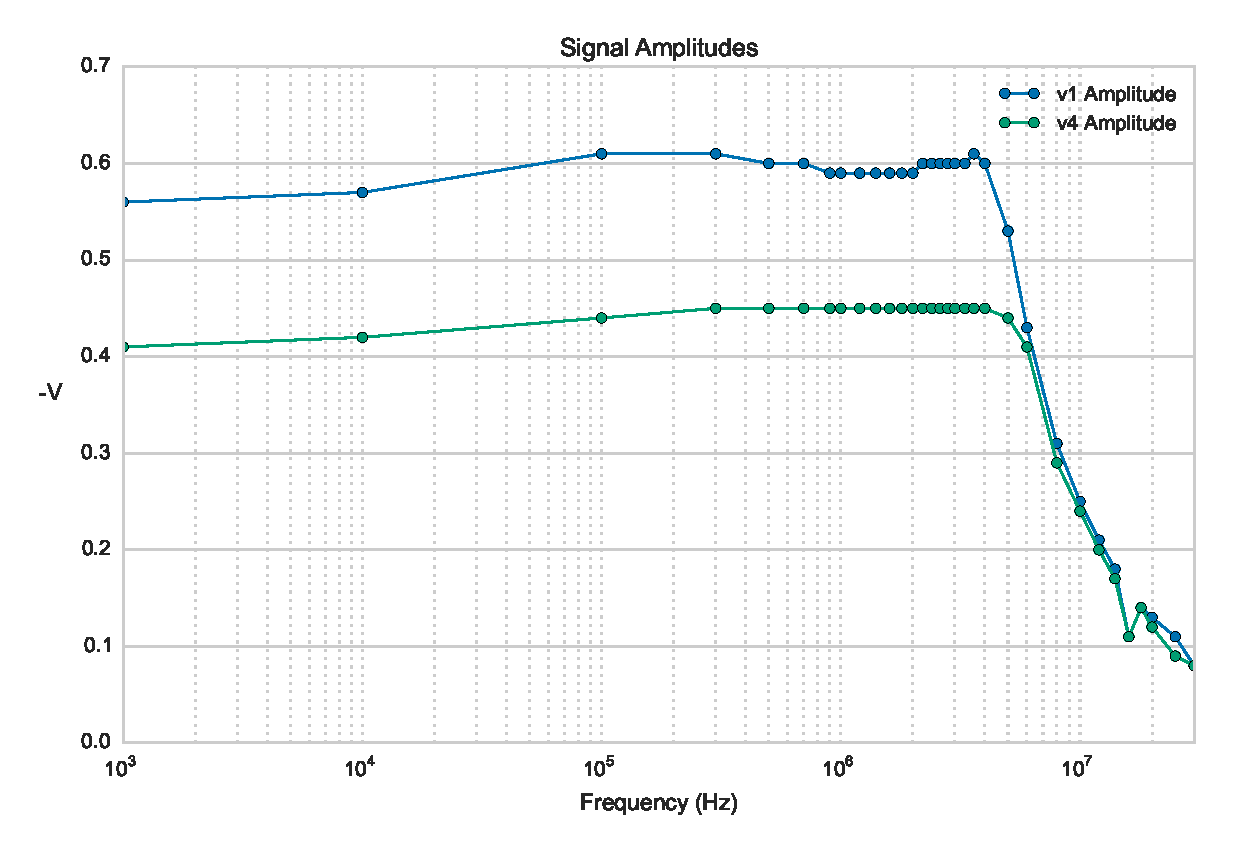
\includegraphics[width=0.5\textwidth]{figures/Test_v4_Amp.eps} 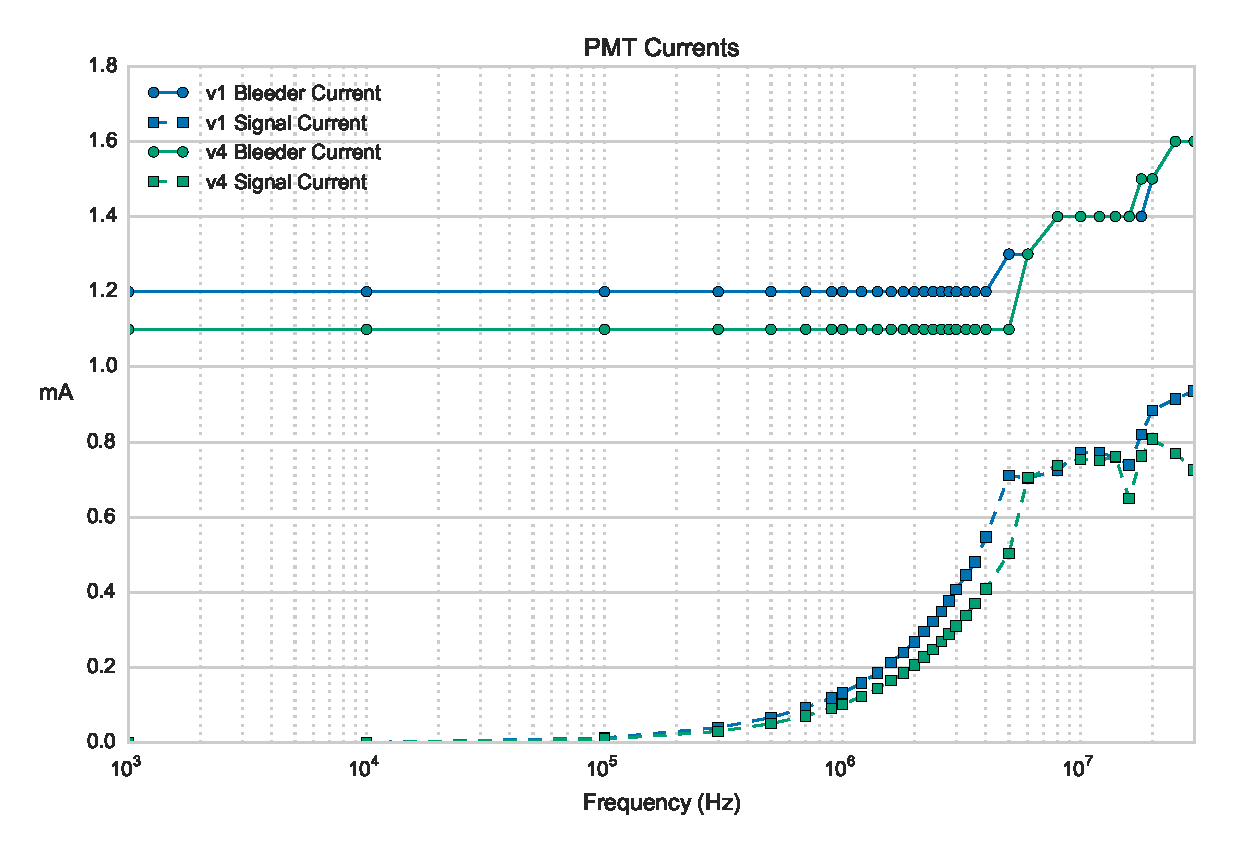
\includegraphics[width=0.5\textwidth]{figures/Test_v4_Current.eps}}}
	\caption{Measurements of the (a) signal amplitudes and (b) bleeder and signal currents in the prototype v1 and prototype v4 PMT bases.}
	\label{fig:test-v4}
\end{figure}

\subsection{Base Comparison Conclusions}

\section{Base Manufacturing and Installation}
